\subsection{What are Graph Databases?}

Graph databases are one of the four most prominent types of NoSQL databases. These are Key-Value, Document oriented, Column databases, and Graph databases.\footnote{S. Priyanka and AmitPal, "A Review of NoSQL Databases, Types and Comparison with Relational Database," International Journal of Engineering Science and Computing, vol. 6, no. 5, pp. 4963-4966, 2016.} This is in contrast to relational databases, where there is only one form of Relational Database which is based on the relational model.\footnote{M. A. Mohamed, "Relational vs. NoSQL Databases: A Survey," International Journal of Computer and Information Technology, vol. 3, no. 03, 2014.} The query language used in graph databases is typically different from that used in relational databases. For example, Cypher is a query language used in Neo4j, a popular graph database, while SQL is used in relational databases. 

Cypher and Neo4j will be used as examples in the comparison with relational databases. Some knowledge of SQL is expected to understand the concepts discussed in this paper.

% tables vs graphs, show an image of a table and a graph
% add image from assets filder
\begin{figure}[ht]
    \centering
    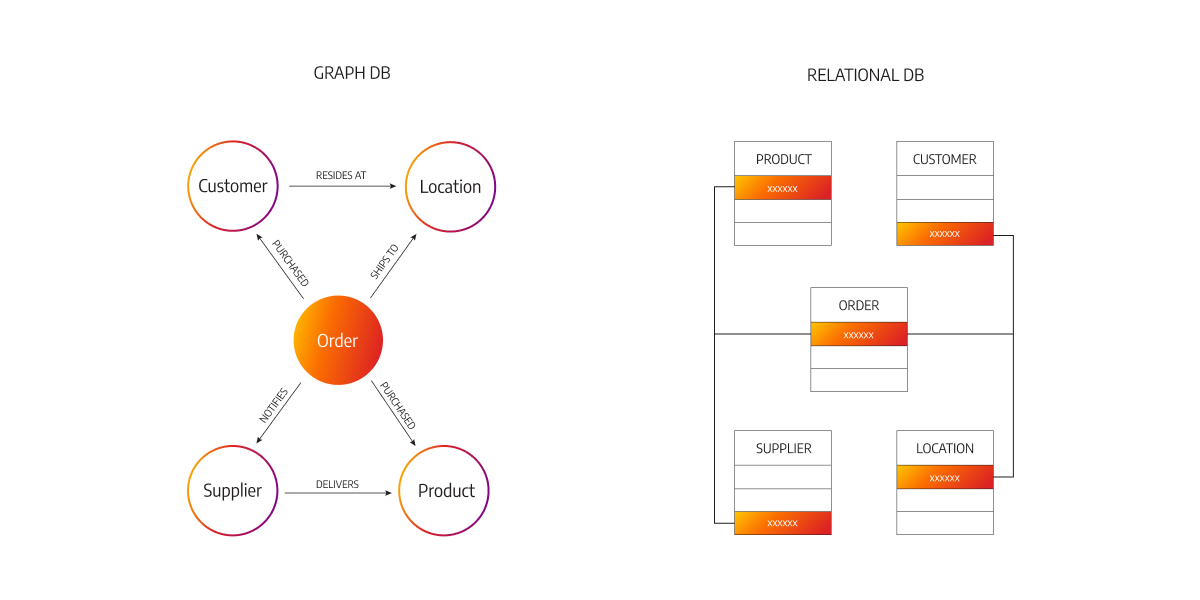
\includegraphics[width=0.7\textwidth]{assets/memgraph-graph-database-vs-relational-database.png}
    \caption{Comparison of graph databases vs. relational databases.\protect\footnote{Image source: Memgraph, \url{https://memgraph.com/blog/graph-database-vs-relational-database}}}
    \label{fig:graph_vs_table}
\end{figure}
In Figure \ref{fig:graph_vs_table}, we see a comparison of graph databases and relational databases. The graph database on the left shows a graph schema, while the relational database on the right shows a relational schema. The graph schema shows nodes and relationships between nodes, while the relational schema shows tables and relationships between tables. 

\begin{figure}[ht]
    \centering
    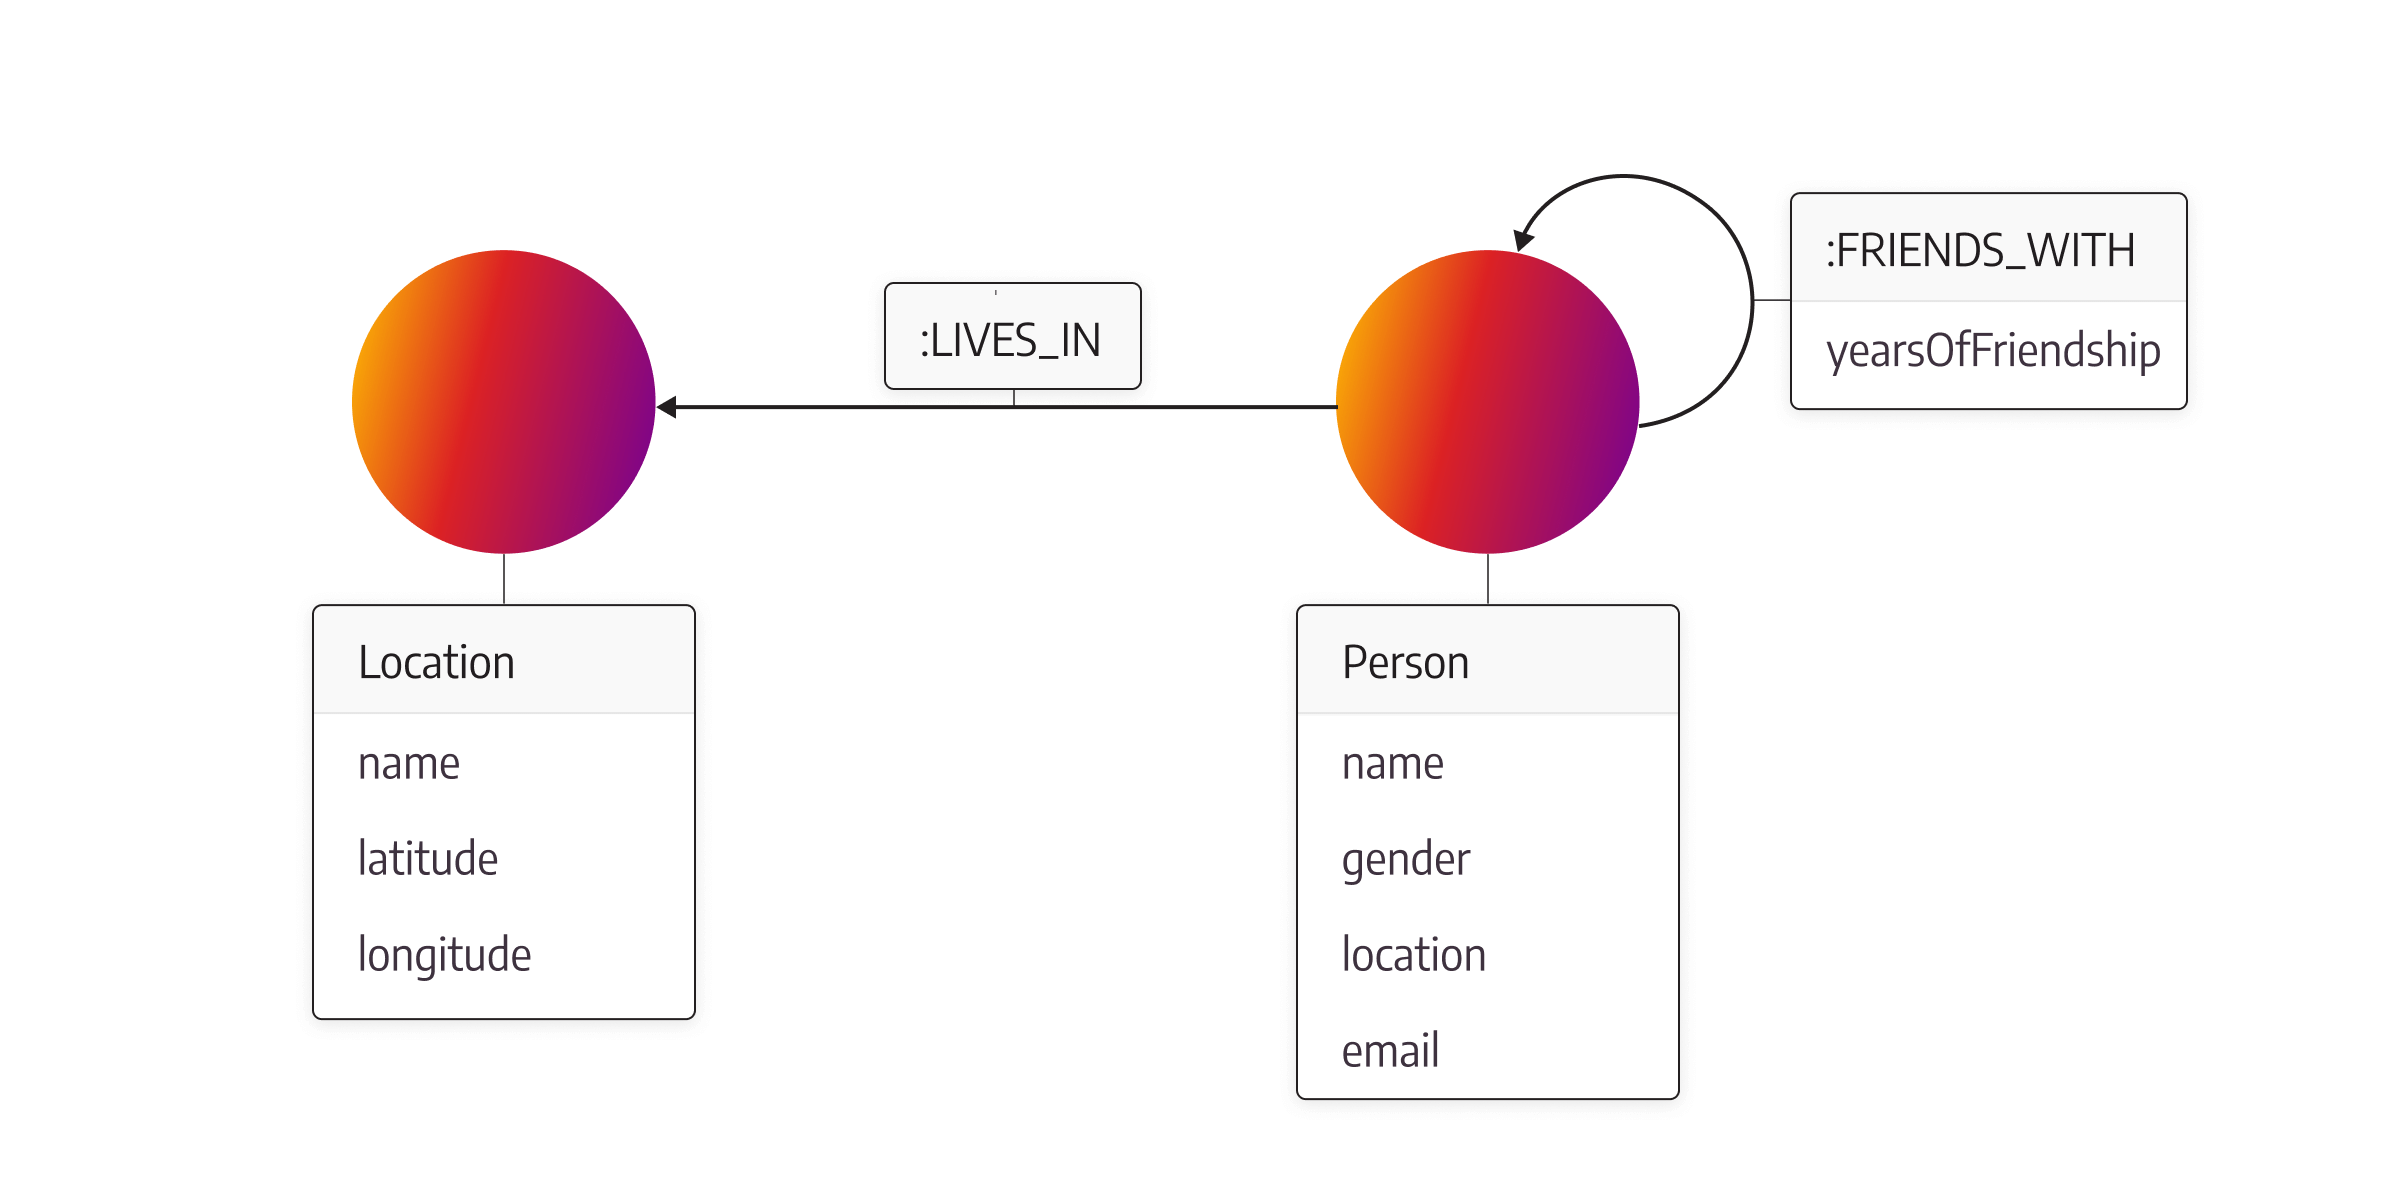
\includegraphics[width=0.7\textwidth]{assets/memgraph-graph-schema.png}
    \caption{Graph Schema.\protect\footnote{Image source: Memgraph, \url{https://memgraph.com/blog/graph-database-vs-relational-database}}}
    \label{fig:graph_schema}
\end{figure}
In Figure \ref{fig:graph_schema}, we see a graph schema. The graph schema shows nodes and relationships between nodes. The nodes represent entities, while the relationships represent the connections between entities. 

\begin{figure}[ht]
    \centering
    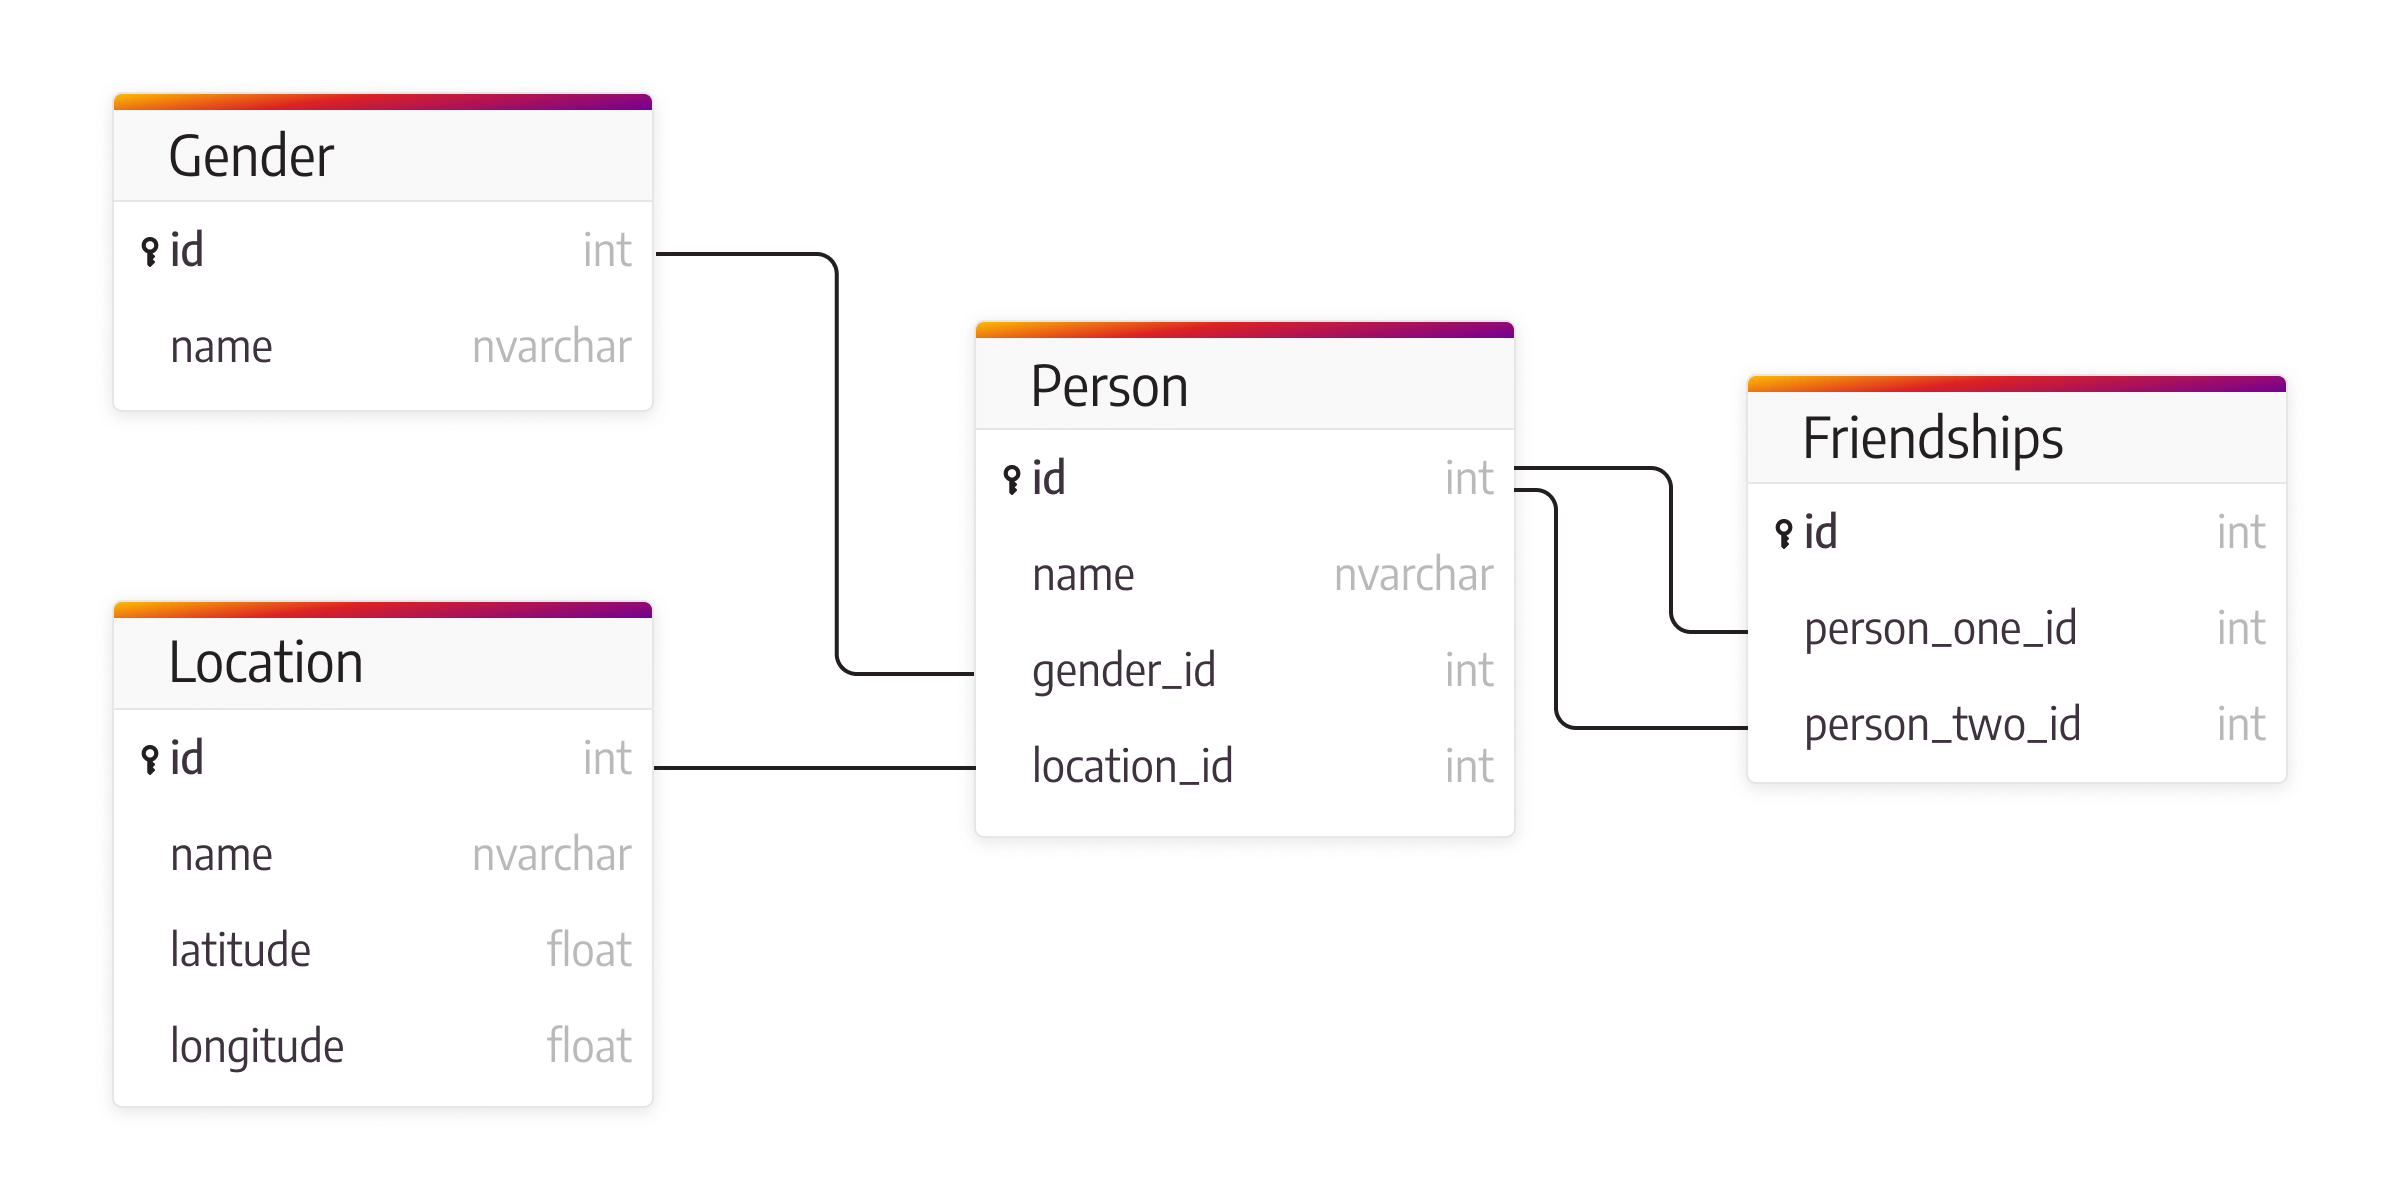
\includegraphics[width=0.7\textwidth]{assets/memgraph-relational-schema.png}
    \caption{Relational Schema.\protect\footnote{Image source: Memgraph, \url{https://memgraph.com/blog/graph-database-vs-relational-database}}}
    \label{fig:relational_schema}
\end{figure}
In Figure \ref{fig:relational_schema}, we see a relational schema. The relational schema shows tables and relationships between tables. The tables represent entities, while the relationships represent the connections between entities.

The purpose of this paper is to compare graph databases with traditional relational databases. This paper is structured as follows: Section 2 provides an overview of graph databases. Section 3 discusses the differences between graph databases and relational databases. Section 4 provides an example showing the differences between the query languages used in graph databases and relational databases. Section 5 concludes the paper and discusses future work.